\iffalse

\subsection{Implementation}

\label{sec:individual}

Feito et. al. \cite{feito2013fast} had noticed that intersection neighborhood can be used for fast classification of faces around that intersection. According to their method, faces adjacent to intersection have neighbors from other primitive(\bm{s}) that define the position and orientation for each other, by which the indicators are determined. However, Feito et. al. did not give detail description of how to implement an exact and robust classification. Their implementation of using vertex coordinates might misclassify faces by numeric errors and fail in degenerate cases. Because geometry connectivity is used, local misclassification can be spread to the neighborhoods, leading to errors in wide ranges.

We develop an classification method that is unconditionally robust and exact based on the idea of using intersection neighborhood information. The neighborhood information is stored in the context component of I-reps during previous stages . In the following, we discuss the conditions that the face to be classified is a triangle. If the face is not a triangle, we select a triangle slice of the face instead, as the whole face is guaranteed to be classified together. Note that the chosen slice should contain the edge where the I-reps lie, by which we compute the new indicators.

Given a face $t_i$ to be classified and an I-rep $\boldsymbol\Gamma$ of intersection on one of $t_i$'s edge, we denote the three corners it as $\bm{v}_{b*}^{0}(t_i), \bm{v}_{b*}^{1}(t_i), \bm{v}_b^2(t_i),$ where the subscript $*$ means the vertices are on the edge where $\boldsymbol\Gamma$ lies. We also denote the context component of $\boldsymbol\Gamma$ as $C_{P_h \backslash P_j}$, meaning $t_i$ is from primitive $M_j$ and intersects primitive $M_h$. From previous discussion (section \ref{sec:ir}){\color{red}{may be more than one}}, we know there are two types of intersection context---face neighborhood and edge neighborhood. In both conditions, the one or two faces involving in the context split the space into two in and out space by its (their) orientation(\bm{s}). We will see that under such division (denoted as $\boldsymbol{D}(C_{P_h \backslash P_j})$), we can compute $\lambda(t_i, P_j)$ exactly.

Since the faces involving in $C_{P_h \backslash P_j}$ is part of primitive $M_j$, the space division $\boldsymbol{D}(C_{P_h \backslash P_j})$ is homogeneous with the space division by $M_j$ in neighborhood of $\bm{\mathcal{I}}$. The basic idea is to choose one point $\bm{v}_x(t_i)$ on $t_i$ close enough to $\bm{\mathcal{I}}$ to compute $\lambda(\bm{v}_x(t_i), P_j)$, and then compute $\lambda(t_i, P_j)$ accordingly. However, the problem is that we cannot find such a $\bm{v}_x(t_i)$ that can be represented exactly, which means robust classification cannot be performed. Fortunately, we observe that we can choose $\bm{v}_b^2(t_i)$, which is not so close to $\bm{\mathcal{I}}$ instead. To illustrate, assume there is another point $\bm{v}_{x'}(t_i)$ inside of $t_i$ that is very close to $\bm{v}_b^2(t_i)$ ({\color{red}{Fig. x}}). Because all inner points of $t_i$ have the same indicator, $\lambda(\bm{v}_x(t_i), P_j) = \lambda(\bm{v}_{x'}(t_i), P_j)$. On the other hand, we find that $\lambda(\bm{v}_{x'}(t_i), P_j)$ and $\lambda(\bm{v}_b^2(t_i), P_j)$ are always equal under division $\boldsymbol{D}(C_{P_h \backslash P_j})$ ({\color{red}{see Appendix \ref{app:profind}}}). Therefore, $\lambda(\bm{v}_b^2(t_i), P_j)$ is equal to $\lambda(\bm{v}_x(t_i), P_j)$ under $\boldsymbol{D}(C_{P_h \backslash P_j})$, and are coherent with $\lambda(t_i, P_j)$ under the division of whole primitive $M_j$. One additional thing is that when $\lambda(\bm{v}_2(t_i), P_j)=on$, then $\lambda(t_i, P_j)$ can be either $same$ or $oppo$. The normal orientation test have to be performed to eliminate such ambiguity.

\fi

\section{Results and Discussion}


\begin{figure}[t]
\centering
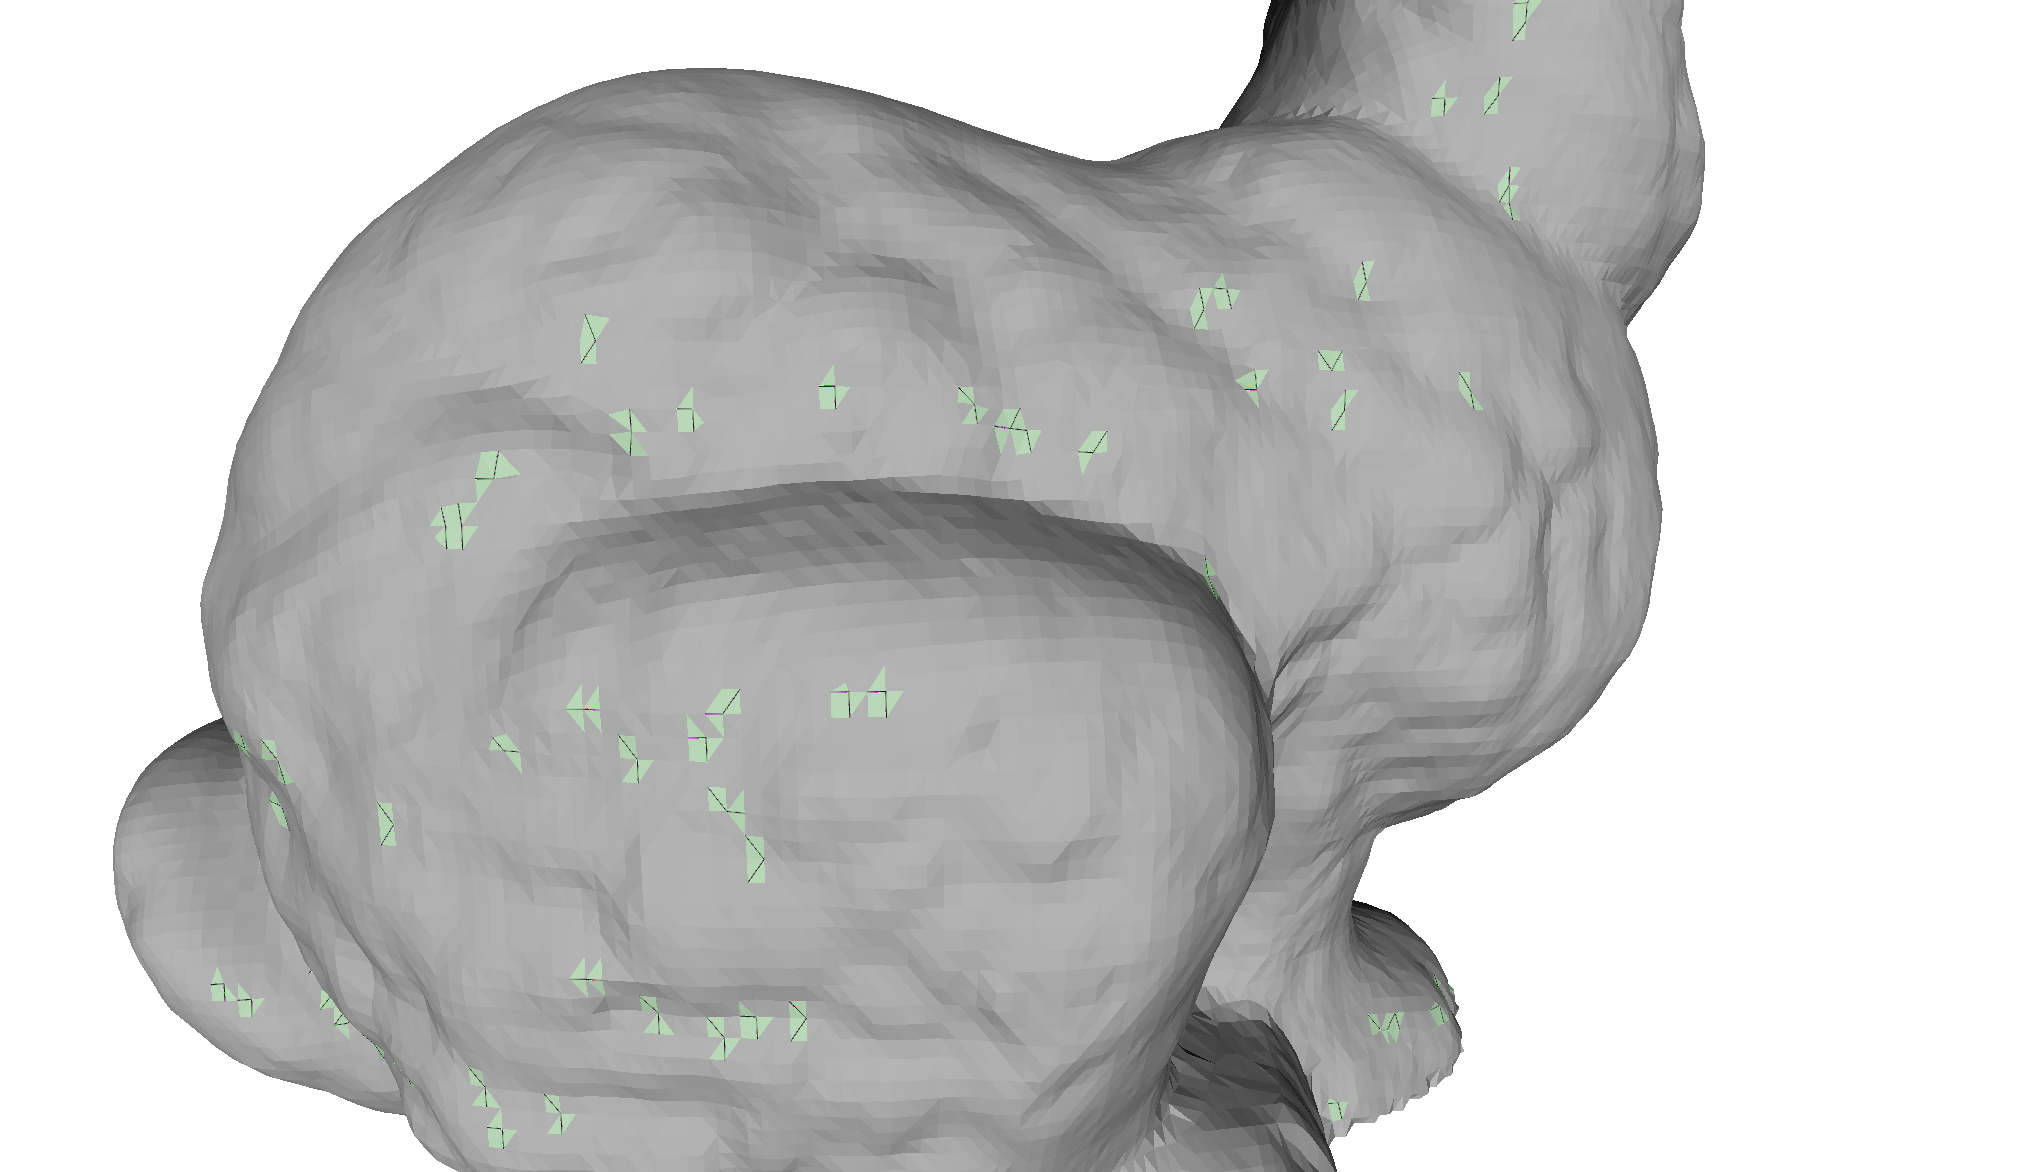
\includegraphics[width=3in]{perturb}
\caption{After perturbation, the self-union of \emph{Bunny} with QuickCSG still suffers from topology problem. The green boundary faces indicate topological deficiencies.}
%
\label{fig:boundaryedge}
\end{figure}

\begin{figure}[t]
\centering
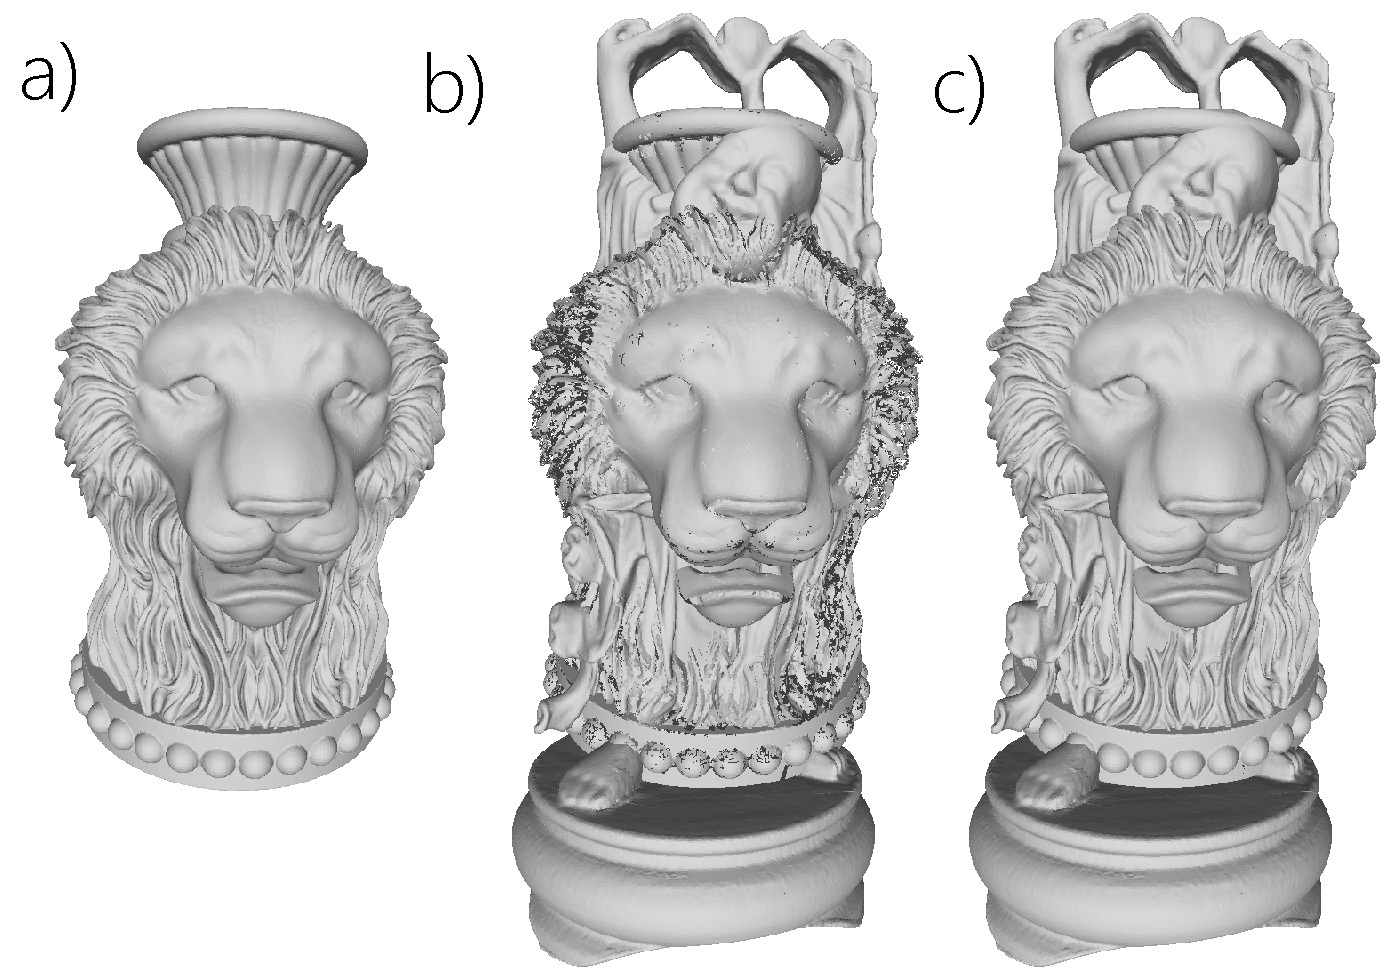
\includegraphics[width=3in]{buddalion}
\caption{ Results from $Budda\cup Lion$: a) incorrect result using CGAL, b) incorrect result using Cork, and c) correct result using our method. }
%.
\label{fig:buddalion}
\end{figure}

%We implemented the proposed method in C++ and tested a series of models on a laptop with Intel Core i5 1.5GHz CPU and 8GB RAM. To prove both the efficiency and robustness, we perform boolean evaluation on various CSGs with different complexity. We also compared our method with several previous works with available implementations, including CGAL \cite{cgal:hk-bonp3-15a}, Maya \cite{Maya2015,barki2015exact},"Cork" \cite{Cork}, "QuickCSG" \cite{douze2015quickcsg}, "Carve" \cite{Carve}, and online service of Campen and Kobbelt's plane-based method \cite{campen2010exact,WebBSP}.

We implemented our proposed method in C++, and tested a series of models on a laptop with an Intel Core i5 1.5 GHz CPU and 8 GB of RAM. To validate the efficiency and robustness of our method, we performed boolean evaluations on various CSGs with different complexities. We also compared our method with several existing methods, including CGAL \cite{cgal:hk-bonp3-15a}, Maya \cite{Maya2015,barki2015exact}, Cork  \cite{Cork}, QuickCSG \cite{douze2015quickcsg}, Carve \cite{Carve}, and online implementations of Campen and Kobbelt��s plane-based method \cite{campen2010exact,WebBSP}.



\subsection{Robustness \& Performance}



\begin{figure}[t]
\centering
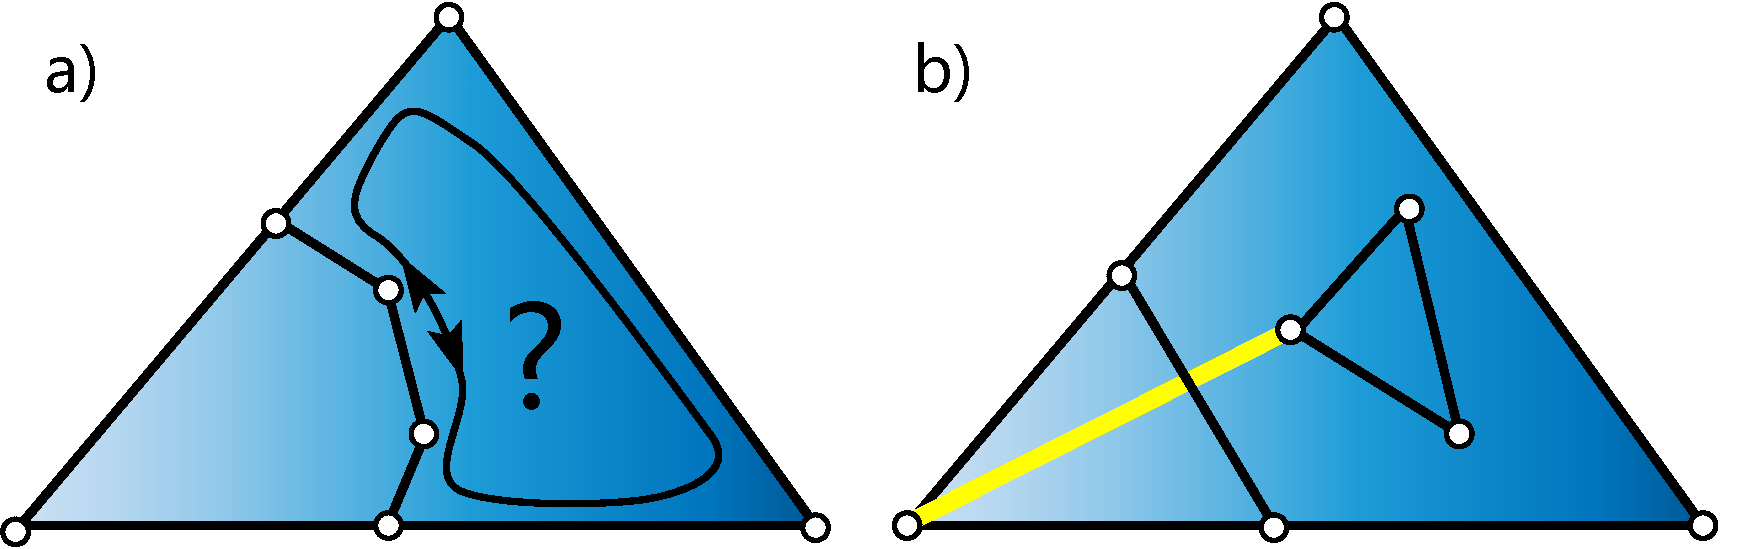
\includegraphics[width=3in]{dual}
\caption{a) There is ambiguity as to the orientation of the loop in this tess-graph. b) When there is more than one connected component in a tess-graph, auxiliary intersections (yellow line) are used to connect the components.}
%a) There is ambiguity with the orientation of the loop in a tess-graph. b) When there are more than one connected component in tess-graph, we use auxiliary intersection (yellow line) to connect the two component. }
\label{fig:dual}
\end{figure}



\begin{table*}[ht]
\caption{Results of self-union evaluation using different methods}
\label{tab:selfunion}
\centering
\begin{tabular}{*{8}{c|}c}%*{4}{>{\centering\arraybackslash}p{35pt}}}
\hline
{No.} & {Model} & {Face Num.} &
CGAL & Maya & Cork & Carve & QuickCSG  & Our Method
\\
\hline\hline
1 & Ball & 360  & \cmark & \cmark & \xmark & \cmark & \xmark & \cmark \\
2 & Head & 2.7k& \cmark & \cmark & \xmark & \cmark & \xmark  & \cmark\\
3 & Bunny & 70k  & \xmark & \cmark & \xmark & \cmark & \xmark  & \cmark\\
4 & Dragon & 277k & \xmark & \xmark & \xmark & \xmark & \xmark  & \cmark \\
\hline
\end{tabular}
\begin{flushleft}
\end{flushleft}
\end{table*}

\begin{table*}[ht]
\caption{Computation time statistics of binary boolean operations (seconds)}
\label{tab:performance}
\centering
\begin{tabular}{*{9}{c|}c}%*{4}{>{\centering\arraybackslash}p{35pt}}}
\hline
{No.} & {Model} & {Face Num. 1} & {Face Num. 2} &
CGAL & Maya & Cork & Carve & QuickCSG & Our Method
\\
\hline\hline
1 & Budda $\cup$ Lion & 1.08M & 400k & - & - & - & - & 3.44 & 6.88\\
2 & Dragon $\cup$ Bunny & 100k & 70k & - & - & - & - & 0.613 &1.70 \\
3 & Armadillo $\cup$ Armadillo2 & 150k & 150k & 487 & 15.4 & 7.00 & 189 & 0.746 & 1.62\\
4 & Horse $\cup$ Corpse & 145k & 499k & - & 38.6 & 12.6 & 1.52k & 0.630 & 1.00 \\
5 & Budda $\cup$ Budda2 & 1.08M & 1.08M & - & - & - & - & 4.84 & -\\
\hline
\end{tabular}
\begin{flushleft}

\end{flushleft}
\end{table*}

\begin{table*}[ht]
\caption{Computation time statistics of the evaluations of large CSGs (seconds)}
\label{tab:performance2}
\centering
\begin{tabular}{*{8}{c|}c}%*{4}{>{\centering\arraybackslash}p{35pt}}}
\hline
{No.} & {Model} & {Face Num.} & {Mesh Num.} &
CGAL  & Cork & Carve & QuickCSG & Our Method
\\
\hline\hline
1 & Sprocket & 11k & 52 & 211  & - & 4.26 & 0.132 & 0.804\\
2 & Ring \& Ball & 146k & 801 & -  & - & 187 & - & 62.6\\
3 & T1 & 80k & 50 & 1.00k & 18.5 & 10.4 & 0.388 & 20.2\\
4 & T2 & 7k & 50 & 2.81k & - & 16.0 & 0.804 & -\\
5 & H & 33k & 42 & - & - & - & 2.22 & -\\
6 & Organic & 219k & 6 & - & 14.3 & 63.1 & 0.580 & 2.75\\
%7 & 6 Budda & - & 43 & - & - & - & - & - & -\\
%8 & Serpent & - & 5 & - & - & - & - & - & -\\
\hline
\end{tabular}
\begin{flushleft}
\end{flushleft}
\end{table*}



\vspace{0.5em}
\noindent\textbf{Self-union}~~~~
%Our method is unconditionally robust for regular set mesh inputs. Even extreme degenerate cases will not lead to failure. To prove that, we tested the self-union of several examples. Table \ref{tab:selfunion} shows whether the tested methods gave a valid outputs. The word 'valid' means the outputs are almost the same with the inputs. In fact, the example models \emph{Bunny} and \emph{Dragon} contain topology deficiencies like self-intersection that cannot perform regular set boolean operations. Despite of that, we find that our method works good in all these cases, indicating the robustness of our method. QuickCSG and Cork failed in all cases, because they cannot deal with coplanar faces. By perturbing one of the operant, the results of QuickCSG are visually OK. However, the topology of their results is messy. We can see hundreds of boundary faces on their results which do not exist in the original model (Fig. \ref{fig:boundaryedge}).
Our method is unconditionally robust for regular set mesh inputs, and even extremely degenerate cases will not lead to failure. To prove this, we tested the self-union of several examples. Table . To prove that, we tested the self-union of several examples. Table  shows whether the methods tested gave valid outputs. Here, the word 'valid' means that the outputs are almost the same as the inputs. The example models \emph{Bunny} $\cap$ \emph{Dragon}  contain topological deficiencies, such as self-intersection, that cannot be processed using regular set boolean operations. Despite this, we found that our method gave good results in these cases, indicating the robustness of our method. QuickCSG and Cork failed in all cases, because they cannot process models with coplanar faces. By perturbing one of the operands, the results of QuickCSG appear visually acceptable. However, the topologies of these results are inaccurate. Hundreds of their boundary faces do not exist in the original model (Fig.  \ref{fig:boundaryedge}).


\vspace{0.5em}
\noindent\textbf{Binary boolean operations}~~~~
%The most common situation of CSG evaluation is to perform boolean operations one by one, since many designers are used to modify models progressively. While our method can evaluate multiple boolean operations once for all, we also compared the performance of binary boolean operations to prove the efficiency. Table \ref{tab:performance} shows the evaluation time of different methods. We can clearly see our method is very fast that is only twice as slower than the fastest non-robust QuickCSG. Other robust methods such as Maya and CGAL are much slower because they use the arbitrary precision arithmetic. Moreover, these robust methods have very strict requirements on the inputs and fragile with topology deficiencies. They simply crash when the inputs are not valid, while our method always tries to give an answer. We also noticed that in (some) very large CSGs, most time is spent on octree construction in our method. It means other stages which involve plane-based geometry take only a small percentage of time, which proves the efficiency of our plane-based algorithms*.
The most common process for CSG evaluation is to perform boolean operations in series. Although our method can evaluate multiple boolean operations simultaneously, we compared the performance of binary boolean operations to determine its efficiency. Table \ref{tab:performance} shows the evaluation times of different methods. These results show that  our method is very fast, and that it is half the speed of the fastest non-robust method, QuickCSG. Other robust methods, such as Maya and CGAL, are much slower, because they use arbitrary precision arithmetic. Moreover, these robust methods have very strict requirements for the inputs, and do not always deal well with topological deficiencies. These methods simply fail when the inputs are not valid, while our method always attempts to provide a result. With (some) very large CSGs, our method spends the most time on octree construction. This means the other stages, which involve plane-based geometry, take only a small percentage of the time. This further demonstrates the efficiency of our plane-based algorithms*.

\vspace{0.5em}
\noindent\textbf{CSGs with large number of meshes}~~~~
%To identify the ability of evaluating large CSG, we also test some CSG with tens or hundreds of meshes. Only QuichCSG and our method can perform multiple boolean operations directly, while others have to decompose CSG trees into binary boolean operations.. We see that the computation time of robust methods like CGAL and Maya is unacceptable long for large CSGs. On the other hand, our method keeps good performance and stability. During our experiments, we noticed sometimes Maya gives the correct results in the first few binary boolean operations, but failed in the later ones. It proves a disadvantage of incremental boolean operation methods---it could accumulate numerical errors which affects the algorithm stability.
To identify the ability of the methods to evaluate large CSGs, we tested some CSGs with tens or hundreds of meshes. Only QuichCSG and our method can perform multiple boolean operations directly. Other methods decompose CSG trees into binary boolean operations. The computation times of robust methods like CGAL and Maya were found to be unacceptably long for large CSGs. Conversely,  our method showed good performance and stability. During our experiments, Maya gave the correct results in the first few binary boolean operations, but failed in the later ones. This demonstrates a disadvantage of incremental boolean operation methods��they can accumulate numerical errors which affect the algorithm��s stability.


\begin{figure*}[!t]
\centering
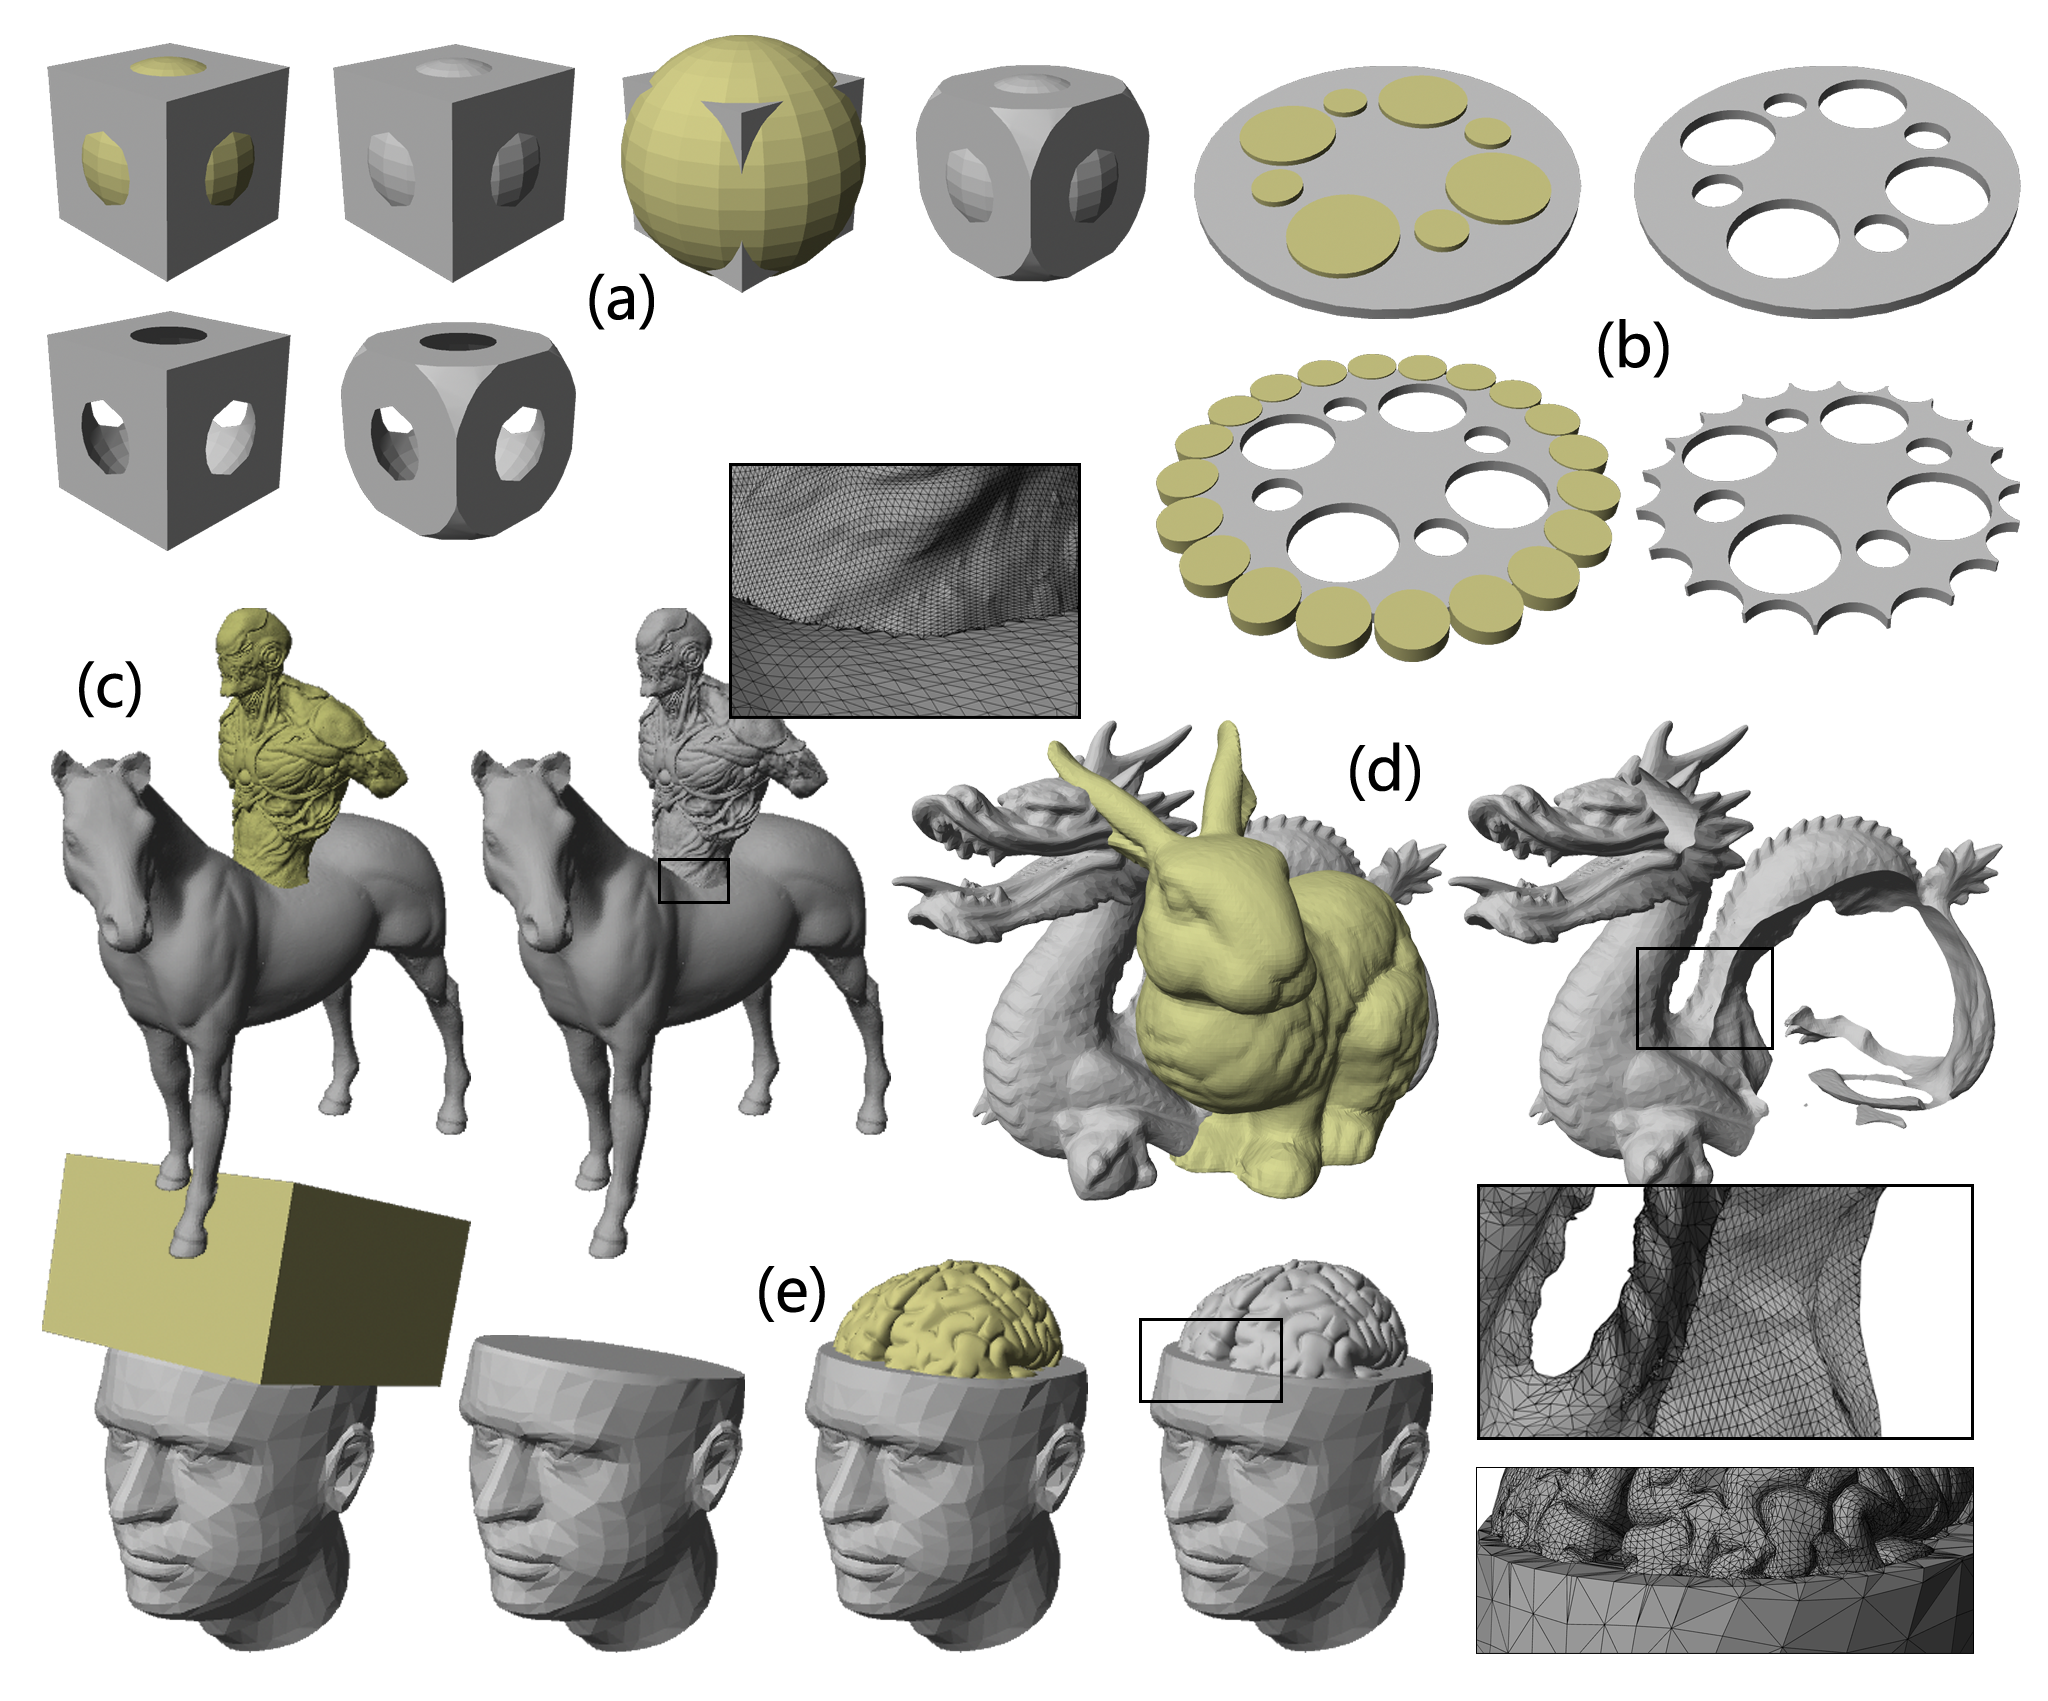
\includegraphics[width=7in]{models}
\caption{***********different models: will be replaced}
\label{fig:models}
\end{figure*}

\subsection{Implementation}
\label{sec:esubroutine}


\vspace{0.5em}
\noindent\textbf{Searching valid loops}~~~~ %In \S\ref{sec:tess}, we claim a valid loops on tess-graph has to be correct with its orientation. However, since tess-graph is undirectional, it is not easy to check whether a loop orientation agrees with the face's (Fig. \ref{fig:dual}a). We observe that the graph connections on the triangle edges have unambiguous directions. Starting from these edges, we can guarantee that the loops have the right orientations. After we find a valid loop, more graph connections will have unambiguous directions because one connection can participate at most two valid loops. In such way, the correct orientation will propagate in a flood-filling way.
Searching valid loops In \S\ref{sec:tess}, we stated that a valid loop on a tess-graph must correspond to its orientation. However, as a tess-graph is nondirectional, it is difficult to check whether a loop orientation agrees with that of the face (Fig. \ref{fig:dual}a). The graph connections on the triangle edges have unambiguous directions. Thus, starting from these edges, we can guarantee that the loops will have the right orientations. After a valid loop is found, more graph connections will have unambiguous directions, because one connection can participate in two valid loops at most. Therefore, the correct orientation will propagate in a flood-filling manner.

\vspace{0.5em}% There is another problem that the tess-graph may not be a connected graph. We avoid this problem by inserting auxiliary intersections into the tess-graph to make it connected. An auxiliary intersection links the corner vertex of triangle face (denoted as $\bm{v}_i$), which is certainly on the outer component, with the vertex on the inner component. The intersection refinement has to be performed again if the auxiliary intersections cross any other intersections. This trick slight obey the principle of no constructions. To guarantee the auxiliary intersection has a valid PBI-rep, we require the vertex from inner connected component generated by intersection between the triangle and an edge (denoted as $\bm{e}_j$) from other meshes---all intersection end points during triangle-triangle intersection are this type. In this way, we get three vertices with exact coordinates ($\bm{v}_i$ and the two end points of $\bm{e}_j$) and can construct an exact plane where the auxiliary intersection lies.
There is no guarantee that the tess-graph will be a connected graph. We solve this problem by inserting auxiliary intersections into the tess-graph, to ensure it is connected. An auxiliary intersection links the corner vertex ( $\bm{v}_i$) of a triangle face which is confirmed to be on the outer component, with the vertex on the inner component. The intersection refinement needs to be performed again if the auxiliary intersections cross any other intersections. This solution is consistent with the principle of no constructions. To guarantee that the auxiliary intersection has a valid PBI-rep, the vertex must be determined from the inner connected component generated by the intersection between the triangle and an edge (denoted as $\bm{e}_j$) from another mesh. All intersection end points of triangle-triangle intersections are of this type. Therefore, we obtain three vertices with exact coordinates ($\bm{v}_i$ and the two end points of $\bm{e}_j$), and, therefore, can construct the plane on which the auxiliary intersection lies.

\vspace{0.5em}
\noindent\textbf{Seed indicator generation}~~~~%In \S\ref{sec:propagation}, we claim that our flood-filling starts from a seed vertex $\bm{v}_0$. While the indicator vector of the seed $\bm{\Lambda}(\bm{v}_0)$ can be generated by point-in-polyhedron test \cite{ogayar2005point} with the octree as acceleration structure \cite{frisken2002simple}, we have simpler strategies by using vertex with known indicators as the seed. We choose the vertex with the max $x$-coordinate as the seed. In this way, its indicators are either $out$ ($in$, if complement is applied on mesh) or $on$. The $on$ indicators are easy to determine in most time. Sometimes exception occurs because of coplanar situation---vertices may not be registered on the mesh even if it is on the mesh. Fortunately, if we carefully choose the right vertex whose neighboring faces are not coplanar, this will not happen.
Seed indicator generation In \S\ref{sec:propagation}, state that flood-filling starts from a seed vertex $\bm{v}_0$. The indicator vector of the seed $\bm{\Lambda}(\bm{v}_0)$ can be generated by a point-in-polyhedron test \cite{ogayar2005point}, using the octree as an acceleration structure \cite{frisken2002simple}. However, a simpler strategy is to use a vertex with known indicators as the seed. The vertex with the maximum $x$-coordinate is chosen as the seed. Its indicators are either $out$ ($in$, if the complement is applied on the mesh) or $on$. The $on$ indicators are generally easy to determine. Exceptions can occur because of coplanar situations��vertices may not be registered on the mesh, even if they are on the mesh. Fortunately, if a vertex is chosen whose neighboring faces are not coplanar, this will be prevented.

\vspace{0.5em} %The indicator vectors can propagate not only among single meshes, but can also between different meshes by the vertices and edges they share. Therefore in most time, we only need one single seed vertex for classification. However, if there are more than two connected components among meshes, we extra seeds to propagate each component. The indicators of the second and later seeds can be computed by point-in-polyhedron tests.
Indicator vectors can propagate among single meshes, and between different meshes across shared vertices and edges. Therefore, in most cases, only a single seed vertex is needed for classification. However, if there are more than two connected components among the meshes, extra seeds are required to propagate each component. The indicators of these additional seeds can be computed by point-in-polyhedron tests.

\vspace{0.5em}
\noindent\textbf{Exporting to float-point number}~~~~
%The vertices of final mesh in our method are represented in either planes or vertex coordinates. While the vertices from the input meshes have there exact coordinates, the vertices newly introduced by intersection between meshes have only P-reps and require round-off when computing coordinates. Though we guarantee the correct topology in the result mesh, such round-off can still cause topology deficiencies. Here we adopt Zhou et al.'s method \cite{zhou2016mesh} to solve it iteratively.
Exporting to float-point number The vertices of the final mesh generated by our method are represented as either planes or vertex coordinates. The vertices originating from the input meshes have exact coordinates, however, the vertices newly introduced by the intersection between meshes have only P-reps, and require rounding-off when computing their coordinates. Although our method guarantees the correct topology in the final mesh, rounding errors can cause topological deficiencies. The method of Zhou et al. \cite{zhou2016mesh} can be used to solve this problem iteratively.

\subsection{Limitations and Future Work}

%We noticed that for CSGs that contains a lot of meshes within small area (e.g., Table. \ref{tab:performance}, \emph{T1}), the performance of our method is poor. This is because in such situations, our method computes many intersections that will not appear as edges in the final mesh, which leads to unnecessary tessellation. Optimization may be explored to avoid such problem.

%The input of our method is limited to regular set meshes. However, recent works claim that the piece-wise wind number (PWN) are more powerful to identify the inside and outside of meshes \cite{zhou2016mesh}.  By using PWN, the input requirements can be extended to so-called PWN meshes that allow topology deficiencies such as self-intersection and multi-component. It would be interesting to extend our method to PWN method in the future.

We found that performance of our method was poor for CSGs that contained a lot of meshes within a small area (Table. \ref{tab:performance}, \emph{T1}). In these cases, our method computes many intersections that will not appear as edges in the final mesh, leading to unnecessary tessellation. Optimization may be explored to minimize this problem.

The application of our method is limited to regular set meshes. However, recent reports have proposed that the piece-wise wind number (PWN) is a more powerful method to identify the insides and outsides of meshes \cite{zhou2016mesh}. The input requirements of our method may be extended to PWN meshes, that allow topological deficiencies, such as self-intersection and multi-components. We believe that this would be an interesting and valuable extension of our work.



\section{Summary}

%In this paper, we proposed a novel method to evaluate CSG models. It is able to efficiently perform unconditionally robust non-incremental boolean operations. The key idea of our approach is to embed P-reps information into B-reps. The P-reps give us the chance to strictly follow the principle of no geometry construction to avoid numerical errors. And the B-reps offer fast neighborhood query to accelerate the processing. Experiments have verified the performance of our method is competitive with state-of-the-art non-robust methods while guarantee robustness.

In this paper, we propose a novel method to evaluate CSG models. This method can efficiently perform unconditionally robust non-incremental boolean operations. The novel component of our approach is to embed P-rep information into B-reps. P-reps allow us to strictly follow the principle of no geometry construction to avoid numerical errors. The use of B-reps enables fast neighborhood queries to reduce the computation time. The experimental results show that the performance of our method is competitive with state-of-the-art non-robust methods, while guaranteeing robustness.
